\chapter{Introduction}

\section{The Game of the Name}

CFT stands for ‘Copious Free Time’: what the author designed, simulated and
built the CFT in.

\section{Aim of this Document}

This document has two aims: one is to document the CFT project in detail, both
for ‘historical’\footnote{‘Historical’ being used here to denote age, not
  quality.} reasons, and because of the author's uncontrollable academic urge
to document his work with reproducibility in mind.

\section{Features}

\subsection{Processor}

\begin{itemize}
\item 16 operation instruction set, plus two composite, bitmap
  instructions.
\item 16 bit word width.
\item All instructions are 16 bits in width.
\item \gls{ABA}.
\item 65,536 word address space.
\item Separate memory and I/O address space.
\item Fully static design. The clock can vary or stop entirely.
\item Partially horizontal microcoded design with vertical fields used
  as failsafe devices to avoid bus contention.
\item The instruction set may be expanded using add-on peripherals or updating microcode.
\end{itemize}

\subsection{Computer and Peripherals}

\begin{description}
\item Eurocard-based backplane design.
\item \textbf{Programmer's front panel.} Provides lights to indicate
  the processor and computer's state at the microcode level and above,
  as well as switches to provide input and modify state.
\item Banked Memory interface for up to 2 MW of memory.
\item Memory cards of 512 kW RAM/ROM.
\item Interrupt controller with 8 interrupt lines.
\item Two to four UART card, including a TTL serial port.
\item Three or six programmable timer card.
\item Real time clock and NVRAM.
\item Two or four IDE disk card.
\item \textbf{Debugging and testing card.} The ‘\gls{DEB}’ board automates
  testing and can act as a simple data collector or logic analyser. It can also
  test peripherals on its own, with the rest of the computer pulled from the
  backplane. This is useful as a safety measure during construction as the
  debugging card is purposefully simple. Detailed documentation on the
  \gls{DEB} board may be found in~\ccf{chap:deb}.
\end{description}

%\begin{floatingfigure}{0.3\columnwidth}
\begin{figure}
  \centering
  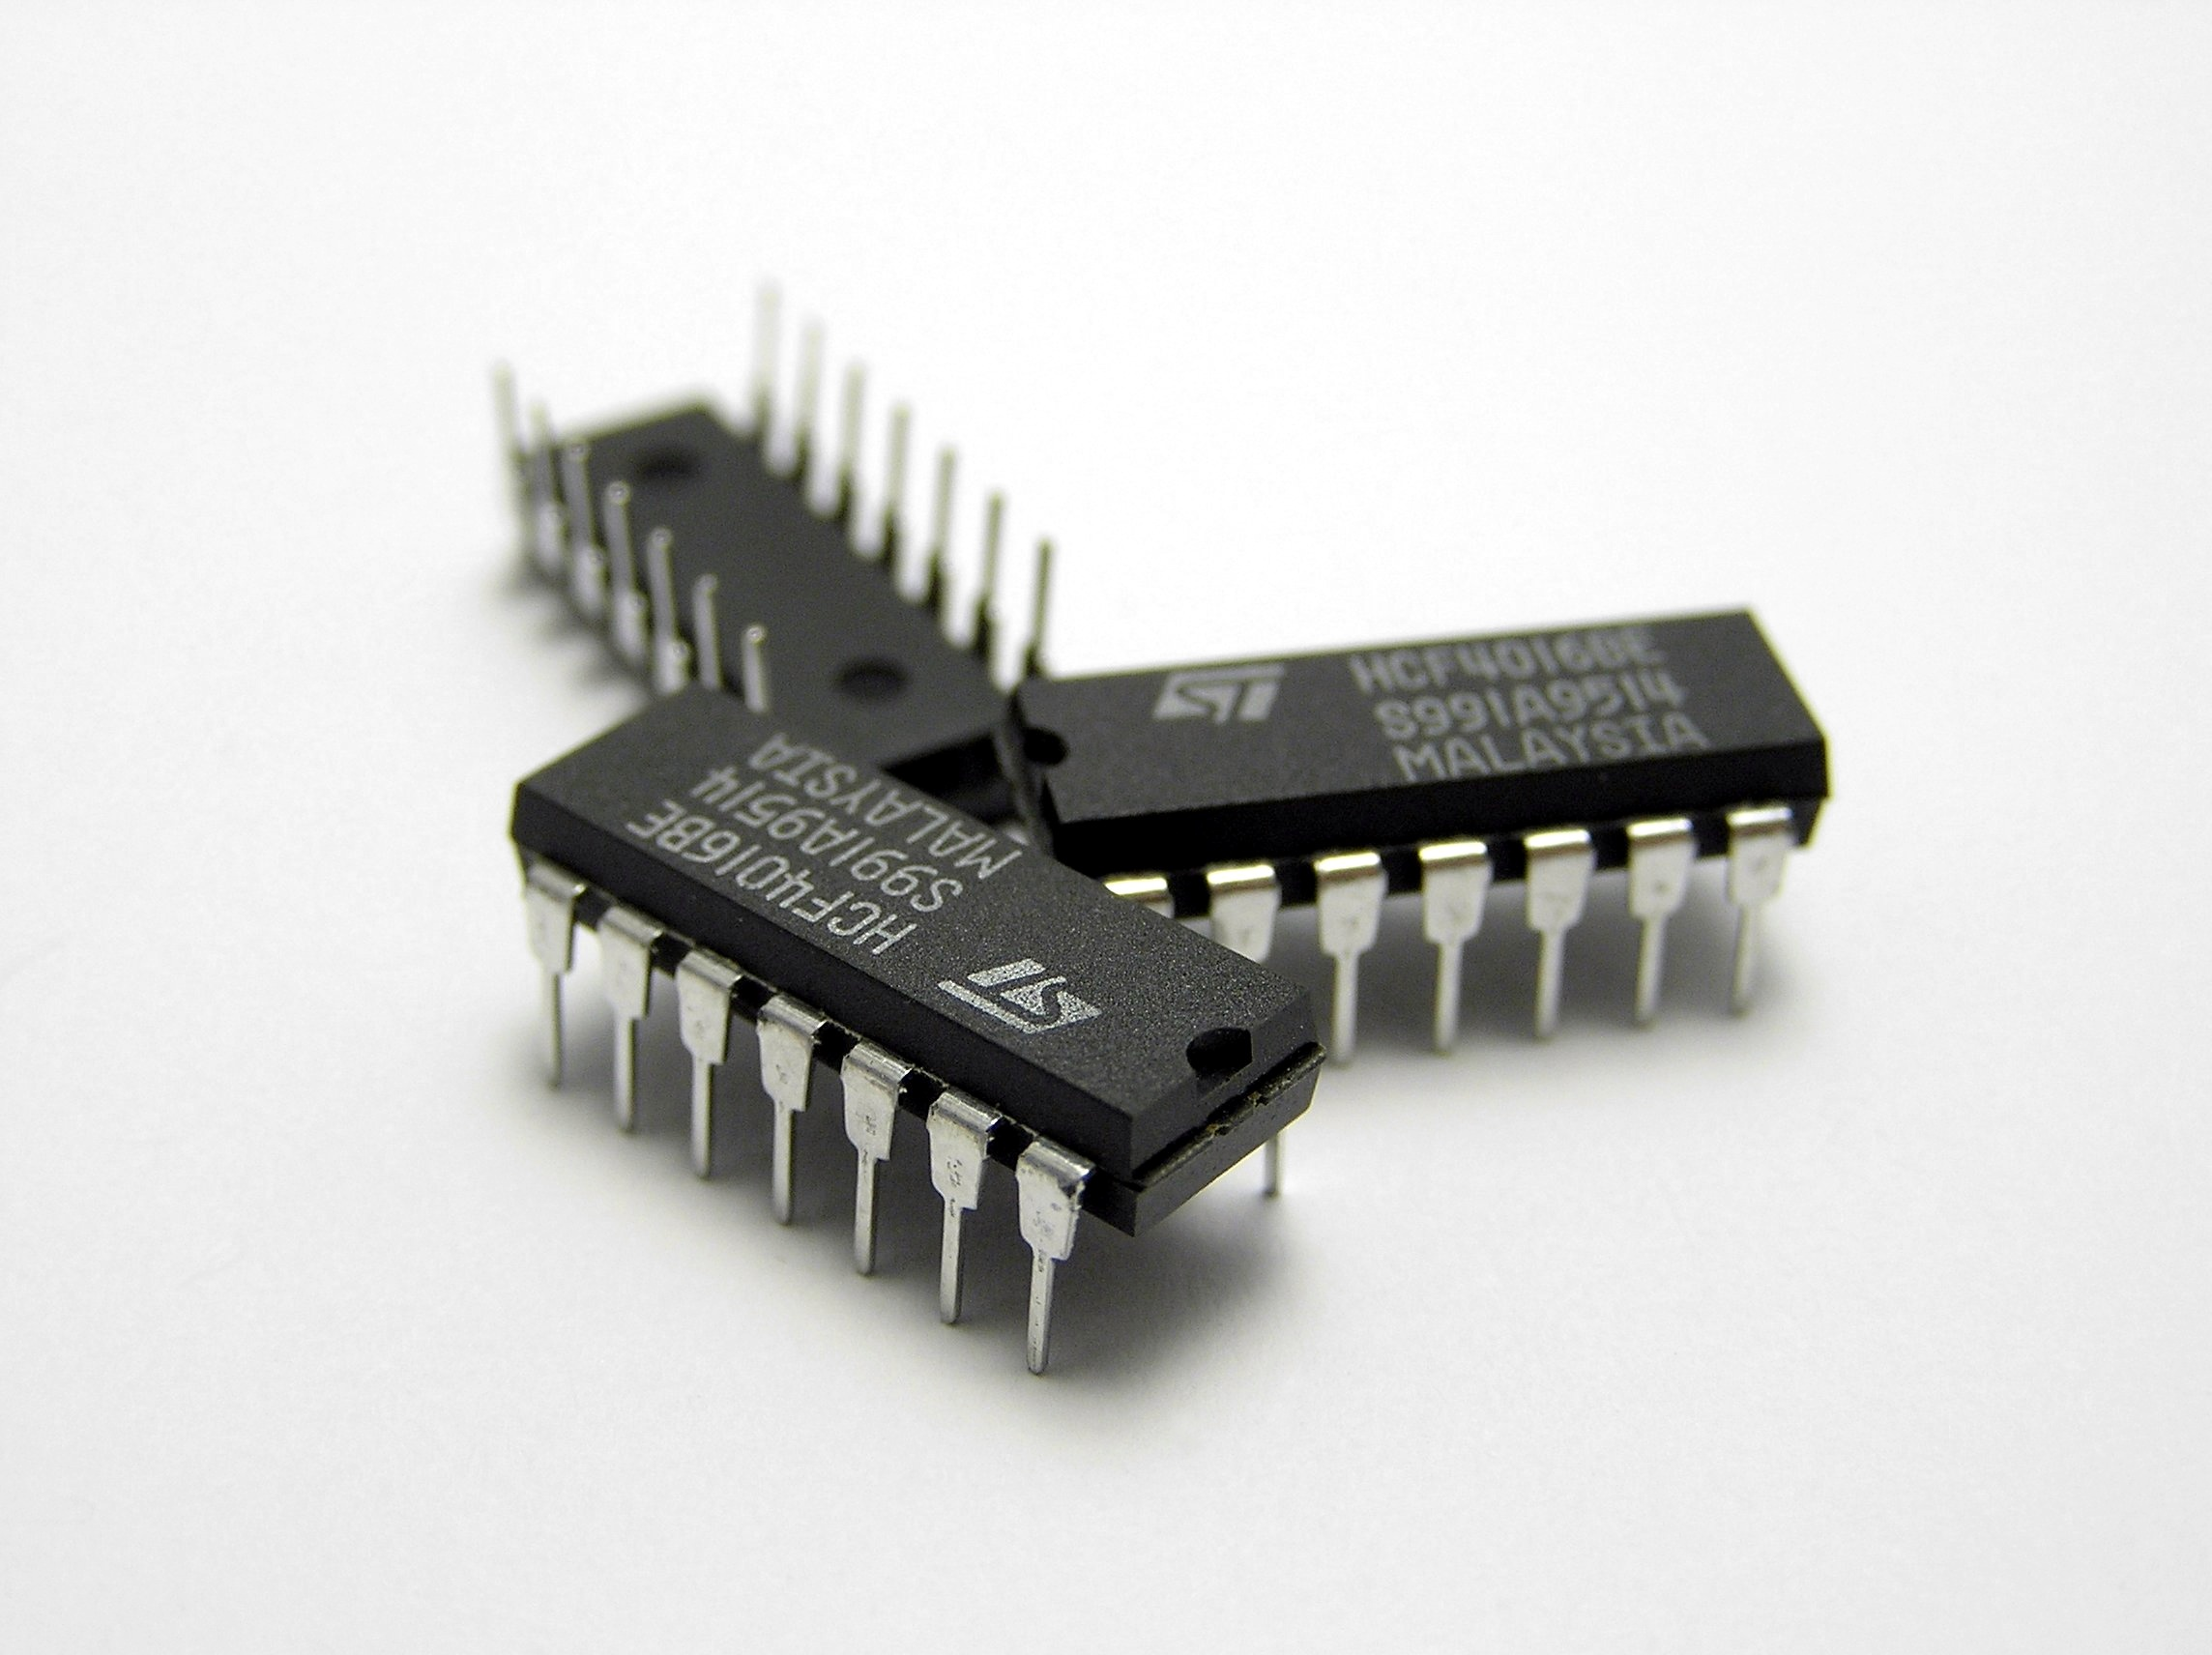
\includegraphics[width=0.5\columnwidth]{figs/Three_IC_circuit_chips.JPG}
  \caption{Three DIP integrated circuits (chips).}
%\end{floatingfigure}
\end{figure}

\subsection{Software}

\begin{itemize}
\item Forth in ROM is used as programming language.
\item Operating System is Forth.
\end{itemize}

\begin{figure*}[t!]
  \centering
  \inputfigure{figure-project-scope}
  %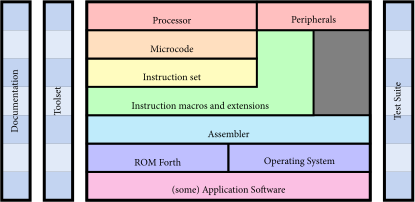
\includegraphics{figure-project-scope.png}
  \caption{\label{fig-projectscope}CFT Project scope and outline.}
\end{figure*}

% End of file.
